%\documentclass[runningheads]{llncs}

\documentclass{article}
\usepackage{nips_2018}


%\usepackage[cmex10]{amsmath, mathtools}
\usepackage{amsmath}
%\usepackage[fleqn]{amsmath}
%\usepackage{amssymb,amsbsy,amsfonts,amsthm}
\usepackage{amssymb,amsbsy,amsfonts}
\usepackage{bm}
\usepackage{enumerate}
\usepackage{url}
\usepackage[ruled,vlined]{algorithm2e}
\usepackage{fancyvrb}
\usepackage{yfonts}
\usepackage{multirow}
\usepackage{multicol}
\usepackage{adjustbox}
%\usepackage[margin=6.5em]{geometry}
\usepackage{makecell} % thicker table separator
\usepackage{booktabs}


\usepackage{subfigure}
\usepackage{wrapfig}
\usepackage{tikz}
%\input{../tikz.conf}

\usetikzlibrary{bayesnet}

%%%%%%%%%%% Box 
\usepackage{calc}%    For the \widthof macro
\usepackage{xparse}%  For \NewDocumentCommand
\newcommand{\tikzmark}[1]{\tikz[overlay,remember picture] \node (#1) {};}


%\input{./header.tex}
%%%%%%%%%% Math
\renewcommand{\text}{\textnormal}
%\newcommand{\pr}{\mathbf{p}}
\newcommand{\pr}{p}
\newcommand{\p}{p}
\newcommand{\E}{\mathbb{E}}
\newcommand{\divkk}{\mathbb{K}}
\newcommand{\entropy}{\mathbb{H}}
\newcommand{\gem}{\mathrm{GEM}}
\newcommand{\Mult}{\mathrm{Mult}}
\newcommand{\DP}{\mathrm{DP}}
\newcommand{\IBP}{\mathrm{IBP}}
\newcommand{\M}{\mathcal{M}}
\newcommand{\V}{\mathcal{V}}
\newcommand{\N}{\mathcal{N}}
\newcommand{\D}{\mathcal{D}}
\renewcommand{\L}{\mathcal{L}}
\newcommand{\mat}[1]{\mathbf{#1}}
\newcommand{\unit}{1\!\!1}
\newcommand{\zij}{z_{i\rightarrow j}}
\newcommand{\zji}{z_{i\leftarrow j}}
\newcommand{\Thetah}{\hat\Theta}
\newcommand{\Phih}{\hat\Phi}
\newcommand{\thetah}{\hat\theta}
\newcommand{\phih}{\hat\phi}

\newcommand\mms[1]{\vcenter{\hbox{$\scriptstyle #1$}}}

%\renewcommand{\Phi}{\mat{\Phi}}


%\date{avril 2015}

%\newtheorem{definition}{Definition}[section]
%\newtheorem{proposition}{Proposition}[section]
%\newtheorem{theorem}{Theorem}[section]
%\newtheorem{corollary}{Corollary}[section]
%\newtheorem{proof}{Proof}[section]


\begin{document}

\title{Online Learning of Stochastic Blockmodels Adapted for Weighted Networks}
	
\maketitle

\begin{abstract}
We propose an online learning algorithm designed to model binary, weigthed, directed or undirected networks. It relies on a probabilistic framework inherited from the mixed-membership stochastic blockmodel. The inference combines the advantages of Variational Inference, in particular to derive stochastic gradient descent of the variational objectives which enables minibatches updates, and Collapse Gibbs Sampling that weaken the assumption made by the classical mean-field approximation of the posterior distribution. We study the convergence of the inference and we evaluate the performance of the models on several real world networks. Our experiments show that our algorithm exhibits fast convergence and have competitive  results on links prediction task especially when the network is partially observed. Futhermore, we show that the weighted MMSB (WMMSB) with an Beta-Gamma priors proposed (WMMSB-bg) signifanctly improves link prediction on most of the weighted networks tested compared to MMSB.
\end{abstract}


\section{Introduction}

Relational data is widespread in many modern applications. From social networks to protein interactions, from physics to linguistics, all interacting objects can be represented as a graph where the objects are the nodes and the interactions the edges. The interest for modelling such networks has naturally increased with the availability of large datasets. Especially in the machine learning literature, that focused on link prediction, dimensionality reduction and data exploration tasks. One of the main challenge in this area is to be able to handle massive networks that emerge from the web. In this paper, we focus on networks that underpin some kind of social relationship such as collaboration or communication networks. In this context, we propose an online learning algorithm that we derived for both binary and count edge covariate, within the framework of Mixed-Membership Stochastic Blockmodel (MMSB).

%%% The type of networks that exists
%Complex networks are graphs that are used to represents real world relationnal information. In computer science, a major network is the web that connects a large amount of data. There is a large diversity in the type of data that can be interconnected, which ca be a set of people in a social plateform, a set of documents linked with hyperlinks, communication networks of email  or more recently a graph of transaction encoded in a blockchain. Outside the web an other important networks is the one made of the scientific collaborations.

%%% The Scalability problem => Sparse Network E/N**2 << 1
%The complexity (time and memory) of batch algorithm are polynomial for graph. Thus, the need of online algorithm, able to update a model as data become available is fundamental for scaling strategy. This can because of the temporality of the data or more simply because the data don't fit in memory. Another source of diversity in networks is the support for labelled and dynamic networks. In this paper we study and propose an algorithm based on latent models with rich priors who scale for complex and massive networks, with labeled edges (weighted networks), and that can be adapted to model the exchangeability of sequences of binary networks (temporal networks).

%
\section{Weighted Networks or Time exchangeability}

% dense - unrealistic
The link prediction models, in the literature \cite{review1,review2}, usually represents networks by a graph $G=(V,E)$ where the edges in the set $E$ are either $0$ or $1$ to account respectively for the absence or the presence of an edge between two nodes. Formally the likelihood of such model is characterized by a Bernoulli density such that $y_{ij} \sim \mathrm{y_{ij} |\theta_{ij}}$. Moreover all of those models are in a setting of static graphs which is formally traduced by the assumption of exchangeability. It means that the joint probability of a graph do not depend on the order of which we observes the nodes. %? $echangeability$

% sparse - real
The main limitation of such models is that they can't handle sparse networks, which is a corollary of the Aldous-Hoover theorem \cite{orbanz2015bayesian}. The models has been said to be misspecified. A way to alleviate this limitation is to weight edges instead of considering binary one. This weighting can be understood, in some way, as smoothing the networks. Additionally, a weighted network is a binary networks where information has bee added under the for of node labeling. The reason why sparsity could be handle this way is because, by considering a weighted networks, it makes all non-edges in a network (0 entries in the adjacency matrix) having a weak contribution to the degree distribution of associated node (see section \ref{todo}). Thus, the inference process can take advantage of this fact because, in sparse networks, most of the interactions are unrealized.

In this paper we will consider the weighted relations as a measure for the number of times each nodes have interacted. Thus, a natural prior for such assumptions is a Poisson distribution. It follows that we will define the likelihood to generate a weighted edge such that $y_{ij} \sim \mathrm{\theta_{ij})}$. Moreover, this representation can take advantage of relational data that arise in various scenario, summarized by the two following:
\begin{itemize}
\item Weighted Networks, where weights represent the \emph{strength} of the relations between individuals,
\item Sum of \emph{snapshot} of binary (or weighted) networks.
\end{itemize}

In the second case the weights can also be seen as a \emph{strength} of connection between individuals, since it represents a count/number of times they interacted together. There is a number of situations where such a case arise. One can think for example to the count of clicks that one user makes during a session. Or the number of time that a individual send a message to another in a social network or again the number of transportation between two cities. Thus modeling weighted networks is a way to take into account the strength of relations that arise in a temporal context, but by keeping the exchangeability assumptions. Or say differently, we loose the time order in which each individual connections took place. That is the reason why we use the term \emph{time exchangeability}.

The use of a Poisson law as an aggregator for single snapshots is primarily justified by the two following fundamental properties \cite{orbanz2012lecture}:
\begin{itemize}
\item{Additivity}: If $K_1 \sim \mathrm{Poisson}(\alpha_1)$ and $K_2 \sim \mathrm{Poisson}(\alpha_2)$ then:
    \begin{equation}
        K_1 + k_2 = \mathrm{Poisson}(\alpha_1 + \alpha_2)
    \end{equation}
\item {Thinning}: The number of successes in a Poisson number of coin flips is Poisson, namely if $K \sim \mathrm{Poisson}(\alpha)$ and $X_1,...,X_2 \sim_{iid} \mathrm{Bern}(p)$, then:
    \begin{equation}
        \sum_{i=1}^K X_i = \mathrm{Poisson}(p\alpha)
    \end{equation}
\end{itemize}

Those two properties of the Poisson distribution constitute the justification of building weighted networks datasets from sequence of either weighted graphs or binary graphs and making inference with Poisson based likelihood.

\section{Model -- WMMSB}
A powerful model for binary exchangeable networks is the Mixed Membership Stochastic Blockmodel (MMSB). In order to keep the strength behind the MMSB models, we propose a generalization of it for weighted networks such as described in the previous section.

The proposed model is a weighted extension of MMSB, named WMMSB. The main design difference is that the likelihood is drawn from a Poisson distribution, and the correlations between the shared classes are drawn from independent Gamma distribution. The models first draw latent class membership for each nodes from a shared Dirichlet distribution. Then for each interactions, each node draw a single membership. The observation level is then draw from Poisson distribution taking is rate parameter according to two classes that summarize the interaction between the two underlying nodes. The observation corresponds to the strength of the relationship. The generative model (along  with the graphical model) is summarized as follows:

\begin{figure}[h]
\begin{minipage}[h]{0.45\linewidth}
\begin{align*}
	&\textrm{For each } i \in \{1, .., N\}  \\
	&\qquad\bm{f}_i \sim \textrm{Dir}(\alpha)\\
	&\textrm{For each }  (m,n) \in \{1,..,K\}^2 \\
	&\qquad\phi_{mn} \sim \mathrm{Gamma}(k,\theta)\\
	&\textrm{For each } (i,j) \in V^2 \\
	&\qquad z_{i \rightarrow j} \sim \mbox{Cat}(\bm{f}_i)\\
	&\qquad z_{i \leftarrow j} \sim \mbox{Cat}(\bm{f}_j)\\
    &\qquad y_{ij} \sim \mathrm{Poisson}(\phi_{z_{i \rightarrow j}z_{i \leftarrow j}})
\end{align*}
\end{minipage}
\begin{minipage}[h]{0.45\linewidth}
	\scalebox{0.88}{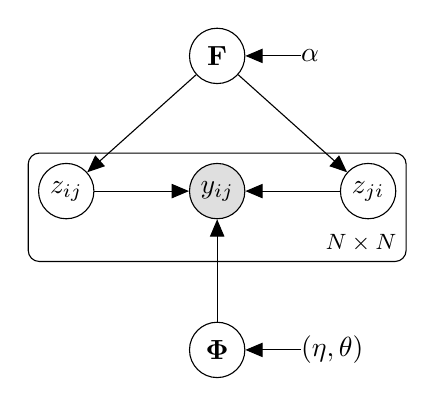
\begin{tikzpicture}
    %\begin{scope}[yshift=0.5cm]
  % Define nodes
  \node[obs]                      (y) {$y_{ij}$};
  \node[latent, left=1.2cm of y] (zi) {$z_{ij}$};
  \node[latent, right=1.2cm of y] (zj) {$z_{ji}$};
  \node[latent, above= of y]    (ibp) {$\mat{F}$};;
  \node[latent, below= of y, yshift=-0.3cm]   (W) {$\mat{\Phi}$};
  \node[const, right=0.7cm of ibp]   (b) {$\alpha$};
  \node[const, right=0.7cm of W]   (sw) {($\eta,\theta$)};

  % Connect the nodes
  \edge {zi,zj,W} {y} ;
  \edge {ibp} {zi,zj} ;
  \edge {sw} {W} ; 
  \edge {b} {ibp} ; 

  % Plates
  \plate {yx} {(zj)(zi)(y)} {$N\times N$} ;
  %\end{scope}
\end{tikzpicture}
}
\end{minipage}
    \caption{Generative models and Bayesian graph of WMMSB.}
\end{figure}

Note that the group membership of each node is context dependent. That is, each node may assume different membership when interacting or being interacted with by different peers. Statistically, each node is an admixture of group-specific interactions. The two sets of latent group indicators are denoted by $\{z_{p\rightarrow q} : p, q \in V\}  =: Z_\rightarrow$ and $\{z_{p\leftarrow q} : p, q \in V\}  =: Z_\leftarrow$. Also note that the pairs of group memberships that underlie interactions need not be equal; this fact is useful for characterizing asymmetric interaction networks. Equality may be enforced when modeling symmetric interactions. \ref{goldenberg2010survey}.

%In the rest of this paper  we will note the set of hyperparameters as $\H = (\alpha, \theta, k)$.

For simplicity, the marginal likelihood (or evidence), takes the following form:
\begin{equation}
    \p(Y | \alpha, \Phi) = \int_F \sum_Z \p(Y| Z, \Phi) \p(Z|F) \p(F| \alpha) dF
\end{equation}

Furthermore, observed links are conditionally independant given the parameters for nodes ($F$) and for classes ($\Phi$) and by marginalizing over the class membership. Thus the likelihood can be written as a matrix decomposition :
\begin{equation}
P(Y | F, \Phi) = \prod_{i,j \in V^2} f_i \Phi f_j^T
\end{equation} 

Unfortunately the evidence is intractable, and conducts the practitioner to resort to approximate inference. In the next section, we propose a Stochastic Collapsed Variationnal inference method.

\section{Inference}

\textcolor{red}{Erics/Chrsitine Note's : Until the double column below wich deal with both network models type, weighted and binary (poisson/bernoulli), the variational derivation holds for both. Just the structure of the Bayesian Graph matter, the familly of the parameter's distribution does not. Furthermore, if the familly distribution of parameters falls into the exponential familly wth conjugate prior, there is closed form updates for the variational inference.}

The Variational Baye's (VB) method is an inference method where the parameters of the Bayesian model, $(F, \Phi, Z)$, are approximated with some free variational parameters $(\nu, \epsilon, \gamma)$. It consists of an iterating algorithm which updates the variational parameters. Those updates are found by maximizing the lower bound arising from the Jensen Inequality. This is equivalent to  minimize the Kullback-Leibler divergence between the variational (posterior) distribution over the variational parameters denoted $q(F, \Phi, Z | \nu, \epsilon, \gamma)$ (we will suppress reference to the variational parameters in the variational posterior for brevity) and the true (posterior) distribution $p(F, \Phi, Z | \tau)$ where $\tau = (\alpha, k, \theta)$ denotes the set of hyperparameters of the model. The evidence lower bound (ELBO) takes the following form :

\begin{equation}
\log p(Y | \tau) = \mathcal{L}(q(F, \Phi, Z)) \geq E_q[\log p(Y, F, \Phi, Z | \tau)] + E_q[\log q(F, \Phi, Z)]
\end{equation}

In classical VB, the variational parameters are taken in the same familly of the true parameters and by assuming that they are fully independent such that :
\begin{equation}
q(F, \Phi, Z) = \prod_{i\in V}q(f_i | \nu_i) \prod_{k,k' \in K^2}q(\phi_{kk'} | \epsilon_{kk'})\prod_{i,j \in V^2}q(\zij, \zji | \gamma_{ij})
\end{equation}

In the Collapsed Variational Baye's (CVB), the assumption on the variational distribution is much weaker. We only assume that the $Z$ variables are mutually independent, thus the variational posterior becomes : 
\begin{align}
q(F, \Phi, Z) &= q(F,\Phi) \prod_{(i,j)\in V^2}q(\zij, \zji | \gamma_{ij}) \\
	&= q(F, \Phi | Z)q(Z)
\end{align}

The ELBO can be split by separating both independent contributions of the variational posterior. Since we do not restrict the form of $q(F, \Phi | Z)$, the ELBO maximum is achieved when the true posterior is reached at $p(F, \Phi | Y, Z,  \tau) = q(F, \Phi | Z)$. The ELBO simplifies in the following collapsed form :
\begin{equation}
\mathcal{L}(q(Z)) = \max_{q(F,\Phi|Z)} \mathcal{L}(q(F, \Phi|Z)q(Z)) = E_q[\log p(Y,Z|\tau)] - E_q[q(Z)]
\end{equation}

The variational parameters are chosen in the same family than the true distribution, thus $q(\zij=k, \zji=k' | \gamma_{ij})$ are multinomial with parameters $\gamma_{ijkk'}$.

Finally, the CVB updates are obtained by minimizing the collapsed ELBO with respect to $\gamma_{ijkk'}$ and it takes the following general form :
\begin{equation} \label{eq:cvb_update}
    \gamma_{ijkk'} \propto \exp \left( E_{q(Z^{\neg ij})} [log(\zij=k, \zji=k' |Y, Z^{\neg ij}, \tau)] \right)
\end{equation}

Where the superscript $\neg ij$ means that the corresponding variables (or counts) are excluded.
This equation is not directly tractable, therefore it is possible to approximate equation \eqref{eq:cvb_update} by noting its relation with the collapse gibbs update. Then,  the closed form expression for the CVB update can be obtain by using a central limit theorem approximation followed by a Taylor expansion.



%\setlength{\columnseprule}{1pt}
%\def\columnseprulecolor{\color{blue}}
%\begin{multicols}{2}[]


The collapse Gibbs update for both models are given by the following equations :

\begin{itemize}
    \item Bernoulli Kernel (MMSB) : \[p(\zij=k, \zji=k' | Y, Z^{\neg ij}, \tau) \propto \quad \frac{ n^{\Phi\neg ij}_{y_{ij}kk'} + \lambda_{y_{ij}}}{n^{\Phi\neg ij}_{\bm{.}kk'} + \lambda_{\bm{.}}} (n^{F\neg j}_{ik} + \alpha_k) (n^{F\neg i}_{jk} + \alpha_{k'})\]
    \item Poisson Kernel (WMMSB) : \[p(\zij=k, \zji=k' | Y, Z^{\neg ij}, \tau) \propto \quad  NB(n^{\Phi\neg ij}_{y_{ij}kk'} + k, \widehat{n}^{\Phi\neg ij}_{y_{ij}kk'} + \theta ) (n^{F\neg j}_{ik} + \alpha_k) (n^{F\neg i}_{jk} + \alpha_{k'})\]
\end{itemize}

Where $NB(a, b)$ represents the pdf of a negative binomial distribution.

The collapse Gibbs Sampler only need to update the counts $n^{n^{\Phi\neg ij}}_{xkk'}, n^{F\neg j}_{ik}, n^{F\neg i}_{jk}$ and $x$ takes its support respectively in $(0,1)$ and $\mathbb{N}$ for MMSB and WMMSB.

In order to compute equation \eqref{eq:cvb_update}, one can approximate the variational distribution with a zero order Taylor expansion under a Gaussian approximation. This is know as the CVB0 algorithm, which gives the following updates :

\begin{itemize}
    \item MMSB : \[ \gamma_{ijkk'} \propto \quad \frac{ N^{\Phi\neg ij}_{y_{ij}kk'} + \lambda_{y_{ij}}}{N^{\Phi\neg ij}_{\bm{.}kk'} + \lambda_{\bm{.}}} (N^{F\neg j}_{ik} + \alpha_k) (N^{F\neg i}_{jk} + \alpha_{k'})\]
    \item WMMSB : \textcolor{red}{Todo}
\end{itemize}

    One can remark the similarity with the Collapse Gibbs update. The difference lives in the counts who now correspond to the means over the variational distribution $q$. The means are approximated trough the central limit theorem of the sum of independent Bernoulli variables with mean $\gamma_{ijkk'}$ such that :
\begin{itemize}
    \item $N^{\Phi}_{xkk'} = \sum_{ij:y_{ij}=x} \gamma_{ijkk'}  \approx   E_q[n^{\Phi}_{xkk'}] $
    \item $N^{F}_{ik}  =  \sum_{j, k'} \gamma_{ijkk'} \approx   E_q[n^{F}_{ik}]$
\end{itemize}


~\\
\textcolor{red}{To complete down here  : ~\\
SCVB update - presents algorithms with noisy gradients and stepsize, minibatch setc.
}



\section{Experiments}

%WMMSB compare it with LDA (a mask)i vs a bipartite networks (Document)
%D (doc) x W (Voc) -- entry count
%
%the bag of word VS the networks representation of document
%* it adds a parameter the document modelization !!!!!!!
 % mote to the Appendix
%\section{Stochastic Block Models}

\begin{figure}[h]
    \hspace*{-3.7em}
\begin{minipage}[h]{0.3\linewidth}
\begin{align*}
	&\textrm{For each } i \in \{1, .., N\}  \\
	&\qquad\bm{f}_i \sim \textrm{Dir}(\alpha)\\
	&\textrm{For each }  (m,n) \in \{1,..,K\}^2 \\
	&\qquad\phi_{mn} \sim \mathrm{Gamma}(\eta,\theta)\\
	&\textrm{For each } (i,j) \in V^2 \\
	&\qquad z_{i \rightarrow j} \sim \mbox{Cat}(\bm{f}_i)\\
	&\qquad z_{i \leftarrow j} \sim \mbox{Cat}(\bm{f}_j)\\
    &\qquad y_{ij} \sim \mathrm{Poisson}(\phi_{z_{i \rightarrow j}z_{i \leftarrow j}})
\end{align*}
\end{minipage}
\begin{minipage}[h]{0.3\linewidth}
	\scalebox{0.88}{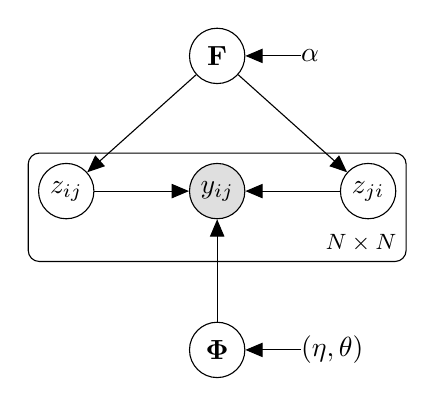
\begin{tikzpicture}
    %\begin{scope}[yshift=0.5cm]
  % Define nodes
  \node[obs]                      (y) {$y_{ij}$};
  \node[latent, left=1.2cm of y] (zi) {$z_{ij}$};
  \node[latent, right=1.2cm of y] (zj) {$z_{ji}$};
  \node[latent, above= of y]    (ibp) {$\mat{F}$};;
  \node[latent, below= of y, yshift=-0.3cm]   (W) {$\mat{\Phi}$};
  \node[const, right=0.7cm of ibp]   (b) {$\alpha$};
  \node[const, right=0.7cm of W]   (sw) {($\eta,\theta$)};

  % Connect the nodes
  \edge {zi,zj,W} {y} ;
  \edge {ibp} {zi,zj} ;
  \edge {sw} {W} ; 
  \edge {b} {ibp} ; 

  % Plates
  \plate {yx} {(zj)(zi)(y)} {$N\times N$} ;
  %\end{scope}
\end{tikzpicture}
}
\end{minipage}
    \caption{Generative models and Bayesian graph of WMMSB.}
\end{figure}

Note that the group membership of each node is context dependent. That is, each node may assume different membership when interacting or being interacted with by different peers. Statistically, each node is an admixture of group-specific interactions. The two sets of latent group indicators are denoted by $Z_\rightarrow = \{z_{p\rightarrow q} : p, q \in V\}$ and $Z_\leftarrow = \{z_{p\leftarrow q} : p, q \in V\}$. Also note that the correlation between classes need not be equal. Equality may be enforced when modeling symmetric interactions. \cite{goldenberg2010survey}.




\section{Inference}





The Variational Bayes (VB) method is an inference method based on the approximation of the Bayesian model's parameters, $(F, \Phi, Z)$, with free variational parameters $(\nu, \epsilon, \gamma)$ usually taken in the same family than the true parameters. It consists of an iterating algorithm which updates the variational parameters by maximizing the lower bound arising from the Jensen Inequality. This is equivalent to  minimize the Kullback-Leibler divergence between the variational (posterior) distribution over the variational parameters denoted $q(F, \Phi, Z | \nu, \epsilon, \gamma)$ (we will suppress reference to the variational parameters in the variational posterior for brevity) and the true (posterior) distribution $p(F, \Phi, Z | \tau)$ where $\tau = (\alpha, \eta, \theta)$ denotes the set of hyperparameters of the model. The evidence lower bound (ELBO) takes the following form :

\begin{align*}
    \log p(Y | \tau) &\geq \mathcal{L}(q(F, \Phi, Z)) \\
    &= E_q[\log p(Y, F, \Phi, Z | \tau)] - E_q[\log q(F, \Phi, Z)] \nonumber \nonumber
\end{align*}

In classical VB, the variational parameters are taken in the same family than the true parameters and by assuming that they are fully independent, this is know as the mean-field approximation :
\begin{align*}
q(F, \Phi, Z) &= \prod_{i\in V}q(f_i | \nu_i) \prod_{k,k' \in K^2}q(\phi_{kk'} | \epsilon_{kk'}) \\
    &\quad \prod_{i,j \in V^2}q(\zij, \zji | \gamma_{ij})
\end{align*}

In the Collapsed Variational Bayes (CVB), the assumption on the variational distribution is much weaker and therefore constitute a better approximation than standard VB \cite{teh2006collapsed}. We only assume that the $Z$ variables are mutually independent, then the variational posterior becomes : 
\begin{align*}
q(F, \Phi, Z) &= q(F,\Phi | Z) \prod_{(i,j)\in V^2}q(\zij, \zji | \gamma_{ij}) \\
	&= q(F, \Phi | Z)q(Z)
\end{align*}

The ELBO can be split by separating both independent contributions of the variational posterior. Since we do not restrict the form of $q(F, \Phi | Z)$, the ELBO maximum is achieved when the true posterior is reached at $p(F, \Phi | Y, Z,  \tau) = q(F, \Phi | Z)$. The ELBO simplifies in the following collapsed form :
\begin{align*}
    \mathcal{L}(q(Z)) &= \max_{q(F,\Phi|Z)} \mathcal{L}(q(F, \Phi|Z)q(Z)) \\
    &= E_q[\log p(Y,Z|\tau)] - E_q[q(Z)]
\end{align*}

The variational parameters are chosen in the same family of distribution than the true distribution, thus $q(\zij=k, \zji=k' | \gamma_{ij})$ are multinomial with parameters $\gamma_{ij}$.

Finally, the CVB update is obtained by maximizing the collapsed ELBO with respect to $\gamma_{ijkk'}$ and it takes the following general form :
\begin{equation} \label{eq:cvb_update}
    \gamma_{ijkk'} \propto \exp \left( E_{q(Z^{\neg ij})} [\log p(\zij=k, \zji=k' |Y, Z^{\neg ij}, \tau)] \right)
\end{equation}

Where the superscript $\neg ij$ means that the corresponding variables (or counts) are excluded.
This equation is not directly tractable, therefore it is possible to approximate equation \eqref{eq:cvb_update} by noting its relation with the collapse Gibbs update. Then,  the closed form expression for the CVB update can be obtained by using a central limit theorem approximation followed by a Taylor expansion.

The Collapse Gibbs Sampler (CGS) for both models are given by the following updates:

%\begin{align*} \label{eq:post_cgs}
%    p(\zij=k, \zji=k' | Y, Z^{\neg ij}, \tau) \propto  \quad & p(y_{ij} | Y^{\neg ij}, Z^{\neg ij}, \zij=k, \zji=k', \tau) \nonumber\\
%    & p(\zij=k, \zji=k' | Z^{\neg ij}, \tau)
%\end{align*}
\begin{align} \label{eq:post_cgs}
    &p(\zij=k, \zji=k' | Y, Z^{\neg ij}, \tau) \propto  \nonumber\\
    & \quad p(\zij=k, \zji=k' | Z^{\neg ij}, \tau) \nonumber \\
    & \quad p(y_{ij} | Y^{\neg ij}, Z^{\neg ij}, \zij=k, \zji=k', \tau)
\end{align}

Both MMSB and WMMSB models had in common the prior over the latent classes which characterise the mixed-membership effect. The update for the left hand part of equation \eqref{eq:post_cgs} represents a reinforcement effect on latent classes membership :

\begin{align*}
    & p(\zij=k, \zji=k' | Z^{\neg ij}, \tau) \propto  \nonumber\\
    & (n^{F\neg j}_{ik} + \alpha_k) (n^{F\neg i}_{jk} + \alpha_{k'}) 
\end{align*}


Both models difference arise from their kernels that are respectively Bernoulli-Beta and Poisson-Gamma distributed for MMSB and WMMSB. The righ part of equation \eqref{eq:post_cgs} are given by the updates in table \ref{table:cgs} :

%\paragraph{MMSB :}
%%    \item MMSB : {\setlength{\mathindent}{0cm} \begin{align*} \quad & p(y_{ij} | Y^{\neg ij}, Z^{\neg ij}, \zij=k, \zji=k', \tau) = \nonumber \\ & \quad  \frac{ n^{\Phi\neg ij}_{y_{ij}kk'} + \lambda_{y_{ij}}}{n^{\Phi\neg ij}_{\bm{.}kk'} + \lambda_{\bm{.}}}\end{align*}}
%    \begin{align*} \quad & p(y_{ij} | Y^{\neg ij}, Z^{\neg ij}, \zij=k, \zji=k', \tau) = \nonumber \\ & \quad  \frac{ n^{\Phi\neg ij}_{y_{ij}kk'} + \lambda_{y_{ij}}}{n^{\Phi\neg ij}_{\bm{.}kk'} + \lambda_{\bm{.}}}\end{align*}
%
%\paragraph{WMSB :}
%\begin{align*} &\quad p(y_{ij} | Y^{\neg ij}, Z^{\neg ij}, \zij=k, \zji=k', \tau) = \nonumber\\& \quad  NB(y_{ij}; n^{Y\neg ij}_{kk'} + \eta, \frac{1}{n^{\Phi\neg ij}_{\bm{.}kk'} + \theta + 1} )\end{align*}
%
\begin{table}[h] \label{table:cgs}
\caption{Gibbs updates for the MMSB and WMMSB kernels.}

    \begin{tabular}{ll}
    \hline
    CGS update    & $p(y_{ij} | Y^{\neg ij}, Z^{\neg ij}, \zij=k, \zji=k', \tau)$ \\
    \hline
    MMSB  & $\frac{ n^{\Phi\neg ij}_{y_{ij}kk'} + \lambda_{y_{ij}}}{n^{\Phi\neg ij}_{\bm{.}kk'} + \lambda_{\bm{.}}}$ \\
    WMMSB & $NB(y_{ij}; n^{Y\neg ij}_{kk'} + \eta, \frac{1}{n^{\Phi\neg ij}_{\bm{.}kk'} + \theta + 1} )$ \\
    \hline
    \end{tabular}
\end{table}


Where $NB(x;a, b)$ represents the pdf of a Negative Binomial distribution parametrized by $(a,b)$.

The collapse Gibbs Samplers only need to update the various counts $n^*$ that emerge from the conjugacy of prior in the *MMSB models. The counts represents the following quantities :
%\begin{align*}
%    &n^{F}_{ik} = \sum_j \delta(\zij=k) + \delta(z_{j\leftarrow i}=k) \qquad\qquad\qquad n^{Y}_{kk'} = \sum_{ij} y_{ij}\delta(\zij=k, \zji=k') \\
%    &n^{\Phi}_{xkk'} = \sum_{ij} \delta(y_{ij}=x, \zij=k, \zji=k') \qquad  n^{\Phi}_{\bm{.}kk'} = \sum_x n^{\Phi}_{xkk'}
%\end{align*}
\begin{align*}
&n^{F}_{ik} = \sum_j \delta(\zij=k) + \delta(z_{j\leftarrow i}=k) \\  
&n^{Y}_{kk'} = \sum_{ij} y_{ij}\delta(\zij=k, \zji=k') \\
&n^{\Phi}_{xkk'} = \sum_{ij} \delta(y_{ij}=x, \zij=k, \zji=k') \\
&n^{\Phi}_{\bm{.}kk'} = \sum_x n^{\Phi}_{xkk'}
\end{align*}

In order to compute equation \eqref{eq:cvb_update}, one can approximate the variational distribution with a zero Taylor expansion under a Gaussian approximation. 

By the central limit theorem, one can compute the expectations of the counts statistics under the variational distribution, that we will refer as $N^* \approx E_q[n^*]$. They are given by a sum of independent variables, where each token is the result of a Bernoulli trial with mean $\gamma_{ijkk'}$. The variational counts statistics can be obtained as follow:

\begin{align} \label{eq:stat_cvb}
    &N^{F}_{ik} = \sum_{j, k'} \gamma_{ijkk'} \qquad\quad  N^{Y}_{kk'} = \sum_{ij} y_{ij}\gamma_{ijkk'} \\
    &N^{\Phi}_{xkk'} = \sum_{ij:y_{ij}=x} \gamma_{ijkk'} \qquad  N^{\Phi}_{\bm{.}kk'} = \sum_x N^{\Phi}_{xkk'}
\end{align}

Under this Gaussian approximation, we can apply a Taylor expansion of equation \eqref{eq:cvb_update}. For simplicity and effectiveness \cite{asuncion2009smoothing}, we propose a zero order approximation, which is know as the CVB0 algorithm and gives the following updates :

\paragraph{MMSB :}
\begin{align*}
\gamma_{ijkk'} \propto  \frac{ N^{\Phi\neg ij}_{y_{ij}kk'} + \lambda_{y_{ij}}}{N^{\Phi\neg ij}_{\bm{.}kk'} + \lambda_{\bm{.}}} (N^{F\neg j}_{ik} + \alpha_k) (N^{F\neg i}_{jk} + \alpha_{k'}) 
\end{align*}

\paragraph{WMMSB :}
\begin{align*}
\gamma_{ijkk'} &\propto NB(y_{ij}; n^{Y\neg ij}_{kk'} + \eta, \frac{1}{n^{\Phi\neg ij}_{\bm{.}kk'} + \theta + 1} ) \\
&\quad (N^{F\neg j}_{ik} + \alpha_k) (N^{F\neg i}_{jk} + \alpha_{k'}) 
\end{align*}

%%% Equation don't fit in table.
%\begin{table}[h] \label{table:cvb}
%\caption{CVB updates for the MMSB and WMMSB kernels.}
%
%    \begin{tabular}{ll}
%    \hline
%    CVB update    & $\gamma_{ijkk'}$ \\
%    \hline
%    MMSB  & $\frac{ N^{\Phi\neg ij}_{y_{ij}kk'} + \lambda_{y_{ij}}}{N^{\Phi\neg ij}_{\bm{.}kk'} + \lambda_{\bm{.}}} (N^{F\neg j}_{ik} + \alpha_k) (N^{F\neg i}_{jk} + \alpha_{k'})$ \\
%    WMMSB & $NB(y_{ij}; n^{Y\neg ij}_{kk'} + \eta, \frac{1}{n^{\Phi\neg ij}_{\bm{.}kk'} + \theta + 1} )(N^{F\neg j}_{ik} + \alpha_k) (N^{F\neg i}_{jk} + \alpha_{k'})$ \\
%    \hline
%    \end{tabular}
%\end{table}


One can remark the similarity with the Collapse Gibbs update. But as the inference is deterministic, it is possible to derive a stochastic gradient in order to prevent batch learning and to scale to large datasets.












We now derive update for a Stochastic Collapsed Variational Inference (SCVB) for the *MMSB models. It is closely related to The Stochastic Variational Inference (SVB)  where online inference is made possible with variational Inference in the exponential family and to \cite{hoffman2013stochastic} which propose general online E-M algorithm for latent model \cite{cappe2009line}. This approach is useful for the two following reasons :

\begin{itemize}
    \item Scale to large datasets : The time complexity becomes linear with the size of the datasets because the algorithm can work with minibatch of an arbitrary size. The memory complexity is drastically save, because only the minibatch content need be loaded to fit a model against the quadratic complexity usually met in networks.
    \item Dynamic scenario : The size of the minibatch can be arbitrary chosen, and could be use in streaming learning scenario, by relaxing the assumptions made on the step size if the Stochastic gradient.
\end{itemize}

The CVB algorithm is resumed by the statistics $N^*$ (see equations \eqref{eq:stat_cvb}). It means that the model parameter can be recovered from those statistics :

\begin{align*}
    \hat f_{ik} &= \frac{N^{F}_{ik} + \alpha_k }{2|V| + \alpha_{\bm{.}}} \\
    \hat \phi_{kk',x} &= \frac{ N^{\Phi}_{x, kk'} + \lambda_x}{N^{\Phi}_{\bm{.}, kk'} + \lambda_{\bm{.}}}  \qquad \mathrm{for}\quad\mathrm{MMSB}\\
    \hat \phi_{kk',x} &= NB(x; N^Y_{kk'} + \eta, \frac{1}{N^{\Phi}_{\bm{.}kk'} + \theta + 1} ) \qquad \mathrm{for}\quad\mathrm{WMMSB}
\end{align*}

For one observations, global statistics are updated by computing the natural gradient of the objective under variational parameter and given by the following steps :
\begin{itemize}
    \item Maximization : The current state is approximately maximized from the update of $\gamma_{ij}$ which optimize the ELBO for the current token,
    \item Expectation : The expected count statistics are updated which propagates the new observations to the noisy gradient. This propagation is controlled by a gradient step size $\rho^{*}_t$ such that $N^{*, t} = (1-\rho_t)N^{*,t-1} + \rho_t \overline N^{*,t}$
\end{itemize}

Where $\overline N$ is the expected statistics computed as if all observations where drawn as the current variational parameters $\gamma_{ij}$. That is the corresponding  expectation for an observations $(ij)$  are given for the different statistics :
\begin{itemize}
    \item $\overline N^{F}_i = R_i \gamma_{ij}$ where $R_i=2|V_i|$ is the total number of relations for a node $i$ in a graph,
    \item $\overline N^{\Phi} = R Y^{(ij)}$ where $R$ is the total number of relations in the network, for a directed graph is $R=|V|^2$, and $Y^{(ij)}$ is $|\mathcal{Y}| K^2$ tensor such that the matrix entries corresponding to the index equal to $y_{ij}$ are set to $\gamma_{ij}$ and the other ones to zeros.
    \item $\overline N^Y = Ry_{ij}\gamma_{ij}$, similar statistics than  $\overline N^{\Phi}$ for weighted networks.
        
\end{itemize}

\begin{itemize}
\item derivation of CVB for Mmmsb And Wmmsb
\item SCVB update for for Mmms And Wmmsb with stratified sampling strategy
\end{itemize}




\section{Related work}
\label{sec:rl}

%\begin{itemize}
%\item on SBM and WSBM (Clauset/peixoto)
%\item on MMSB familly (Airoldi/Blei/Mimmo/Gopalan) and SVB
%\item on PFA (Poisson Factor Analysis) and Gamma Processes (Zhou etc).
%\item on SCVB (Foulds). (they show that scvb is similar to EM+map on made the links with online EM of (Cappé and Moulines)
%\end{itemize}
In social networks, the presence of a tie between two entities generally indicates that there is a relationship between them and in recent years, researchers proposed various methods to predict the presence or absence of such interaction. However, in many applications, it is the intensity of the relationship that is important. So, for example in epidemiology, it is not enough to know that two people have been in contact but it is also necessary to know the frequency of these contacts to know whether there is a risk of contagion or not. Similarly, in the field of transport, it is not enough to know that there is a motorway or an airline between two cities to analyze the population flows between them, it is also necessary to know the number of vehicles or passengers that goes from the first one to the other. In the field of economy and finance, to know if a company risks being absorbed by another it is not enough to know that the second took shares in the capital of the second but it is also necessary to know how much. This intensity of the relationship is generally modeled as a weight and the network is represented by a weighted graph. Unfortunately, in practice it is often easier to observe the interaction than to measure it. For this reason, there has been a lot of work devoted to link prediction \cite{Liben2007, Zaki2011,  Martinez2016}  %Wang2014
and less to edge weight prediction in social networks.


Like for link prediction, to solve the weight prediction, there are two main approaches, similarity-based and likelihood-based methods \cite{Lu2011}. The methods belonging to the first familly assume that the similarity between two nodes is correlated with their interaction strength. For instance, using this hypothesis, Zhao \textit{et al.} propose to predict missing links and their weights by extending unweighted similarity indices to weighted ones \cite{Zhao2015}. Zhu \textit{et al.} also introduce a method where the estimation of the weights is based on neighbor sets \cite{Zhu2016}.
The second approach formulates the problem in a probabilistic framework and includes extended versions of generative models, initially introduced to learn the network formation process, in particular, the stochastic block model (SBM) \cite{Karrer2011} \textit{CL :ref  Karrer ou Nowicki and Snijders?}.  
However, these models suffer from several limitations notably they consider that a node can  belong to only one class, which is not realistic in real networks and, secondly the inference algorithm is not able to tackle large size networks. The models and inference process presented in this paper aim to overcome these limits. 


The original MMSB model was proposed in \cite{airoldi2009mixed} with a variational inference scheme. The inference process was later extended with stochastic variational inference in \cite{gopalan2013efficient} and structured variational inference in \cite{kim2013efficient} for scalability purposes. Stochastic variational inference has been applied with a collapsed variational objective for the latent Dirichlet allocation model \cite{foulds2013stochastic}\sout{. To} \textit{and to} our knowledge, it is the first time that stochastic and collapsed variational inference are coupled in the context of stochastic block models. \textit{However, the previous models have been designed for link prediction and not for weight prediction.  }

\textit{Weighted versions of the stochastic block model have been intoduced firstly in \cite{mariadassou2010} and then in} \cite{aicher2014learning} who proposed WSBM. WSBM can be seen as a special case of our WMMSB model  in which nodes are constrained to belong to only one latent class \textit{whereas our model allows each node to belong to several classes}. More recently, an extended version of WSBM  model has been presented  in which different kernels can be used to model different types of weights \cite{peixoto2018nonparametric}. An efficient MCMC method is used for inference. If this type of models is interesting, it nevertheless relies again on the assumption that a node belongs to only one class, which may be inappropriate for real world networks. Furthermore, unlike MMSB models, the lack of a hierarchical prior structure does not allow one to rely on efficient non-parametric extensions (hence the use of costly model selection techniques for non-parametric versions). 

Similar to our model, count processes with Poisson distributions and Gamma conjugate priors have been studied \sout{by different authors} \textit{notably by Zhou et al.} \cite{zhou2012augment, zhou2015negative}. The relation of such processes with Negative Binomial processes is well-known and has been highlighted by these authors who applied  these processes for topic modeling, \sout{as} \textit{with} the Beta-Gamma-Gamma-Poisson model (EPM) (\cite{zhou2012beta}) that relies on MCMC inference. They also applied them for  overlapping community detection and link prediction \cite{zhou2015infinite}. The main difference between this model and WMMSB is that the former factorizes counts as Poisson variables of a sum of latent factors while, in WMMSB, counts are factorized as a convex sum of Poisson variable depending on class memberships.

Thus, the main theoretical contribution of this article is two-fold: firstly, we propose a mixed-membership stochastic block model, called WMMSB-bg, for weighted networks allowing nodes to belong to several classes, and secondly we \sout{show how to learn this model on large networks with a stochastic collapsed variational inference algorithm} \textit{design an efficient stochastic collapsed variational inference algorithm able to handle large size networks}.

%
%This work intersects with several groups of related works:
%
%First, the recent advance on Stochatistic Variationnal inference have made it possible to scale bayesian model to bigger dataset and to do online learning which enable a low memory footprint. This inference have first been proposed for topic modeling [1][2] before being adapted for the MMSB model with an adaptation to discover overllaping communities [3] [4],
%
%Nevertheless, the previous works only study the case of (undirected) binary networks.
%
%In [5] the author proposed an efficient inference algorithm for weigthed networks, based on a MCMC algorithms. The model is an extension of the SBM. Those models assumed that the class don't overllap. (I still have to dive into to understand how his inferecne works...) (does it allow online learning ? )
%
%Finally, SVB has been combined with CVB inference for topic modelling to propose a improoved over SVB. [6]
%
%This paper combines the different advantage of those works to propose a Online learning algorithm to models networks that can be weighted, with overllaping classes, directed or undirected.
%


\section{Experimental validation}
\label{sec:exps}

We evaluated the performance of the above models on several real world weighted networks, both directed and undirected. Theirs characteristics and properties are summarized in Table \ref{table:corpus} and detailed descriptions are available in the online Koblenz network collection\footnote{http://konect.uni-koblenz.de/networks/}. For both astro-ph and hep-ph datasets, we used the cleaned versions available in the  graph-tool framework.
%The aim of these experiments is to illustrate the advantage of the online inference and to evaluate the performances of the models.
%This evaluation is based on a missing weight prediction task using the MSE score. 
 For all the datasets, we built a test set by extracting randomly 20 percent of the edges of the network and about the same amount of non-linked pairs of nodes. The remaining data constitutes the training set. We repeated this sampling 10 times with different seeds to cross validate our results. The average values (and standard deviations) computed on the ten sets are reported as final results.

\begin{table*}[t]
\bgroup
\def\arraystretch{1} % 1 is the default, change whatever you need
	
\caption{Datasets networks used to train the models. Type A is for co-authorship, type C is for communication, type H is for hyperlinks and type L is for lexical network.}

\begin{tabular}{lrrrrcrrrr}
%\Xhline{2\arrayrulewidth}
\toprule
 Datasets     &   Nodes &   Edges &   Density & Directed  &    Diameter &   \multicolumn{3}{c}{Weights}  	& type     \\
 \cmidrule(l){7-9}  &   &   	  &   		  & 		  &  		   	&  mean & std  & max             \\
%\hline
\midrule
 astro-ph      &   16706 &  121251 &     0.001    & False    &       14 &   1.8& 3.3 & 306      & A  \\
 cond-mat      &   16726 &   47594 &     0.000    & False    &       18 &   3.1& 7.2& 544      & A  \\
 hep-th        &    8361 &   15751 &     0.000    & False    &        1 &   5.2& 16& 1226      & A  \\
 netscience    &    1589 &    2742 &     0.002    & False    &        2 &   2.2& 1.9 &33       & A  \\
 manufacturing &     167 &    5783 &     0.209    & True     &        3 &  14.3& 44.9&1458    & C  \\
 fb\_uc        &    1899 &   20296 &     0.006    & True     &        4 &   2.8& 4.7& 98       & C  \\
 enron         &    87273  & 320154   &  0.0000   & True     &       15 &   3.4& 12.4&3904    & C  \\
 wiki-link     &  100312   & 887426   & 0.0001    & True     &       14 &   1.7& 3.0& 185      & H  \\
%\Xhline{2\arrayrulewidth}
\bottomrule
\end{tabular}


\egroup
\label{table:corpus}
\end{table*}

In the remainder, for the MMSB, WMMSB and WMMSB-bg models, the gradient step parameters  $\tau$ and $\kappa$ were fixed respectively to  $1024$ and $0.5$, the burn-in period $T_{burnin}$ to $150$; for stratified sampling, $M$ was set to $50$, the size of $s_0^{i,m}, \, 1 \le m \le M$ being equal to the number of nodes to which $i$ is not connected to divided by $M$. For MMSB, the hyperparameters $\lambda_0$ and $\lambda_1$ were set to $0.1$. For WMMSB, $r$ et $p$ were set to $1$ ??? and for WMMSB-bg the hyperparameters were set to  $c_0=10$, $r_0=1$, $c=100$ and $\epsilon=10^{-6}$. The number of latent classes $K$ was fixed to $10$ for all models and the latent-class hyperparameters $\alpha_k$ to $\frac{1}{K}$. The implementation of these models is available online\footnote{https://github.com/***/*** (anonymized)}. For deciding when to stop the inference process, 10\% of the training set used serves as a validation set on which the log-likelihood is computed after each minibatch iteration. When the increase of the log-likelihood, averaged over the last 20 measures, is less than 0.001, the inference is stopped. The log-likelihood of a given set of observations $\D_{set}$  is given by:
%
\begin{equation*}
\log p(\D_{set}) = \sum_{i,j \in \D_{set}} \log p(y_{ij} | \phih_{kk'}) p(k|\thetah_i) p(k'|\thetah_j).
%\log p(\D_{test}) = \sum_{i,j \in \D_{test}} \log p(y_{ij} | \phih_{kk'}) p(k|\thetah_i) p(k'|\thetah_j)
\end{equation*}
%

Predicting links and predicting weights on links are too different tasks, and there is no guarantee that a model performing well on one task will perform well on the other. We nevertheless assess the behavior of the weighted mixed-membership model we have introduced in the context of these two tasks to fully illustrate its performance, however giving more emphasis to weight prediction.

\subsection{Link prediction}

We want to illustrate here how the MMSB and WMMSB-bg models behave for link prediction. In addition to these models, we consider here two standard link prediction models, the stochastic block model, referred to as SBM, and its weighted extension, referred to as WSBM. For these two models, the microcanonical stochastic block model implementation of \cite{peixoto2018nonparametric} has been used since it integrates an efficient MCMC inference method for the stochastic block model family.  In all models, the number of classes is set to $K=10$. 

As usual, the missing link prediction task is evaluated with the AUC-ROC score. For weighted models, we simply predict here a link through the probability that an edge exists between two unobserved nodes $(i,j)$ belonging to the test set, namely:
\[
p(y_{ij} \geq 1 | \Bs{\Thetah}, \Bs{\Phih}) = 1 - \sum_{kk'} \thetah_{ik} \thetah_{jk'} e^{-\phih_{kk'}}
\]

%Variational inference, used here for MMSB models, and MCMC, used for SBM models, lead to different performance, the latter usually yielding better models than the former \cite{asuncion2009smoothing}. Indeed, despite the fact that the MMSB models considered here rely on more realistic assumptions regarding the distribution of nodes over latent classes, the approximations made on the likelihood for scalable inference purposes penalize MMSB models when it comes to prediction accuracy. This said, the strong averaging step of the stochastic gradient descent allows for faster convergence so that, as the models are more realistic, they may yield better performance when the amount of training data is limited. This is indeed what we observe in practice.

Table~\ref{table:roc} summarizes the results obtained with the above mentioned models when using 10\% and 100\% of the training data. As one can note, using all training data, SBM outperforms WSBM on 5 datasets and is the best performing model when the complete training set is used. This can be attributed to the fact that SBM directly aims at predicting links, unlike the weighted models, and does so via MCMC inference, which is known to yield accurate estimate when there is sufficient data. Interestingly, there is an important degradation for SBM models when only 10\% of the training set is used. MMSB models are more stable in this aspect, showing that the stochastic variational inference used in MMSB models allows one to learn a correct model with few data.

\begin{table*}[t]
\centering
	
\caption{Comparison of MMSB, WMMSB-bg, SBM and WSBM in terms of AUC-ROC when using 10\% and 100\% of the training data.}

%\resizebox{12cm}{!}{
\resizebox{\textwidth}{!}{

\begin{tabular}{lllll|llll}
\toprule
&   \multicolumn{4}{c}{10\%} &   \multicolumn{4}{c}{100\%}   \\
\cmidrule(l){2-5} \cmidrule(l){6-9}   & MMSB & WMMSB-bg & SBM & WSBM & MMSB & WMMSB-bg & SBM & WSBM   \\
%\hline
\midrule
astro-ph      & \textbf{708} $\pm$ 3  & 700 $\pm$ 30           & 594 $\pm$ 16 & 586 $\pm$ 9           & \textbf{716} $\pm$ 11 & 710 $\pm$ 18          & 701 $\pm$ 6           & 705 $\pm$ 5 \\
hep-th        & \textbf{617} $\pm$ 11 & 579 $\pm$ 12           & 480 $\pm$ 9  & 482 $\pm$ 26          & 675 $\pm$ 8           & 676 $\pm$ 8           & \textbf{779} $\pm$ 10 & 714 $\pm$ 7 \\
moreno\_names & 680 $\pm$ 72          & \textbf{707} $\pm$ 29  & 571 $\pm$ 29 & 594 $\pm$ 30          & 738 $\pm$ 33          & 739 $\pm$ 7           & \textbf{862} $\pm$ 7  & 859 $\pm$ 11 \\
fb\_uc        & 732 $\pm$ 127         & \textbf{827} $\pm$ 8   & 726 $\pm$ 20 & 788 $\pm$ 18          & 784 $\pm$ 140         & 850 $\pm$ 20          & \textbf{902} $\pm$ 2  & 896 $\pm$ 2 \\
digg\_reply   & 485 $\pm$ 178         & \textbf{651} $\pm$ 127 & 551 $\pm$ 47 & 582 $\pm$ 35          & 482 $\pm$ 204         & \textbf{744} $\pm$ 15 & 728 $\pm$ 26          & 717 $\pm$ 17 \\
slashdot      & 519 $\pm$ 193         & \textbf{820} $\pm$ 6   & 721 $\pm$ 66 & 732 $\pm$ 81          & 634 $\pm$ 181         & 791 $\pm$ 11          & 830 $\pm$ 16          & \textbf{834} $\pm$ 12  \\
enron         & 459 $\pm$ 289         & 875 $\pm$ 14           & 870 $\pm$ 80 & \textbf{923} $\pm$ 14 & 529 $\pm$ 256         & 835 $\pm$ 8           & 799 $\pm$ 20          & \textbf{853} $\pm$ 63  \\
wiki-link     & 491 $\pm$ 242         & 739 $\pm$ 73           & 848 $\pm$ 4  & \textbf{850} $\pm$ 4  & 432 $\pm$ 185         & 785 $\pm$ 8           & \textbf{925} $\pm$ 2  & 915 $\pm$ 3 \\
prosper-loans & 548 $\pm$ 284         & \textbf{752} $\pm$ 11  & 466 $\pm$ 57 & 455 $\pm$ 44          & 434 $\pm$ 274         & \textbf{727} $\pm$ 30 & 500 $\pm$ 4           & 504 $\pm$ 6 \\
\bottomrule
\end{tabular}
}

% 10 100
%\begin{tabular}{lllll|llll}
%\toprule
%&   \multicolumn{2}{c}{MMSB} &   \multicolumn{2}{c}{WMMSB-bg} &   \multicolumn{2}{c}{SBM} & \multicolumn{2}{c}{WSBM}   \\
%\cmidrule(l){2-3} \cmidrule(l){4-5} \cmidrule(l){6-7}\cmidrule(l){8-9}  & 10 & 100 & 10 & 100 & 10 &  100 & 10 & 100   \\
%%\hline
%\midrule                              
%astro-ph        &  \textbf{708} $\pm$ 3    & \underline{716} $\pm$ 11          & 700 $\pm$ 30            &  710 $\pm$ 18   &   594 $\pm$ 16   &  701 $\pm$ 6               &   588 $\pm$ 12           & 705 $\pm$ 5  \\
%hep-th          &  \textbf{617} $\pm$ 11   & 675 $\pm$ 8           & 579 $\pm$ 12            &  676 $\pm$ 8    &   480 $\pm$ 9    &  \underline{779} $\pm$ 1               &   497 $\pm$ 29            & 716 $\pm$ 9  \\
%moreno\_names   &  680 $\pm$ 72            & 738 $\pm$ 33          & \textbf{707} $\pm$ 29   &  739 $\pm$ 7    &   571 $\pm$ 29   &  \underline{862} $\pm$ 7               &   588 $\pm$ 25            & 862 $\pm$ 10 \\
%fb\_uc          &  732 $\pm$ 127           & 784 $\pm$ 14          & \textbf{827} $\pm$ 8    &  850 $\pm$ 20   &   726 $\pm$ 20   &  \underline{902} $\pm$ 2               &   787 $\pm$ 15            & 896 $\pm$ 2  \\
%digg\_reply     &  485 $\pm$ 178           & 482 $\pm$ 204         & \textbf{651} $\pm$ 127  &  744 $\pm$ 15   &   551 $\pm$ 47   &  728 $\pm$ 26              &   584 $\pm$ 34            & 714 $\pm$ 17 \\
%slashdot        &  519 $\pm$ 193           & 634 $\pm$ 181         & \textbf{820} $\pm$ 6    &  791 $\pm$ 11   &   721 $\pm$ 66   &  830 $\pm$ 16              &   699 $\pm$ 79            & \underline{833} $\pm$ 13 \\
%enron           &  459 $\pm$ 289           & 529 $\pm$ 256         & \textbf{875} $\pm$ 14   &  835 $\pm$ 8    &   870 $\pm$ 80   &  799 $\pm$ 20              &   866 $\pm$ 45            & \underline{842} $\pm$ 51 \\
%wiki-link       &  491 $\pm$ 242           & 432 $\pm$ 185         & 739 $\pm$ 73            &  785 $\pm$ 8    &   848 $\pm$ 4    &  \underline{925} $\pm$ 2               &   \textbf{853} $\pm$ 4    & 914 $\pm$ 4  \\
%prosper-loans   &  548 $\pm$ 284           & 434 $\pm$ 274         & \textbf{752} $\pm$ 11   &  \underline{727} $\pm$ 30   &   466 $\pm$ 57   &  500 $\pm$ 4               &   455 $\pm$ 44  	       & 505 $\pm$ 5  \\
%
%\bottomrule
%\end{tabular}
          
          
          





% 5 20 100

%&   \multicolumn{3}{c}{MMSB} &   \multicolumn{3}{c}{WMMSB-bg} &   \multicolumn{3}{c}{SBM} & \multicolumn{3}{c}{WSBM}     \\
%\cmidrule(l){2-4} \cmidrule(l){5-7} \cmidrule(l){8-10}\cmidrule(l){11-13}  & 5 & 20 & 100 & 5 & 20 & 100 & 5 & 20 & 100 & 5 & 20 & 100   \\

%astro-ph        &  686 $\pm$ 7    & 720 $\pm$ 8    & 716 $\pm$ 11   & 684 $\pm$ 25 & 690 $\pm$ 40  &  710 $\pm$ 18   &    505 $\pm$ 9  &  627 $\pm$ 5   &  701 $\pm$ 6   &  538 $\pm$ 31  &    626 $\pm$ 9   & 705 $\pm$ 5  \\
%hep-th          &  583 $\pm$ 13   & 655 $\pm$ 6    & 675 $\pm$ 8    & 558 $\pm$ 9  & 630 $\pm$ 21  &  676 $\pm$ 8    &   498 $\pm$ 6   &  506 $\pm$ 13  &  779 $\pm$ 1   &  513 $\pm$ 24   &    545 $\pm$ 29  & 716 $\pm$ 9  \\
%moreno\_names   &  674 $\pm$ 43   & 740 $\pm$ 18   & 738 $\pm$ 33   & 664 $\pm$ 39 & 697 $\pm$ 33  &  739 $\pm$ 7    &   478 $\pm$ 59  &  698 $\pm$ 25  &  862 $\pm$ 7   &  457 $\pm$ 38   &    709 $\pm$ 9   & 862 $\pm$ 10 \\
%fb\_uc          &  723 $\pm$ 109  & 728 $\pm$ 140  & 784 $\pm$ 14   & 790 $\pm$ 20 & 846 $\pm$ 11  &  850 $\pm$ 20   &   590 $\pm$ 43  &  846 $\pm$ 13  &  902 $\pm$ 2   &  679 $\pm$ 27   &    855 $\pm$ 7   & 896 $\pm$ 2  \\
%digg\_reply     &  491 $\pm$ 150  & 486 $\pm$ 195  & 482 $\pm$ 204  & 667 $\pm$ 73 & 723 $\pm$ 31  &  744 $\pm$ 15   &   528 $\pm$ 51  &  677 $\pm$ 13  &  728 $\pm$ 26  &  554 $\pm$ 22   &    659 $\pm$ 26  & 714 $\pm$ 17 \\
%slashdot        &  537 $\pm$ 177  & 538 $\pm$ 186  & 634 $\pm$ 181  & 801 $\pm$ 13 & 822 $\pm$ 6   &  791 $\pm$ 11   &   712 $\pm$ 66  &  775 $\pm$ 72  &  830 $\pm$ 16  &  731 $\pm$ 64   &    733 $\pm$ 28  & 833 $\pm$ 13 \\
%enron           &  555 $\pm$ 300  & 576 $\pm$ 301  & 529 $\pm$ 256  & 862 $\pm$ 15 & 876 $\pm$ 9   &  835 $\pm$ 8    &   900 $\pm$ 3   &  898 $\pm$ 39  &  799 $\pm$ 20  &  887 $\pm$ 48   &    916 $\pm$ 29  & 842 $\pm$ 51 \\
%wiki-link       &  389 $\pm$ 192  & 505 $\pm$ 230  & 432 $\pm$ 185  & 749 $\pm$ 43 & 725 $\pm$ 87  &  785 $\pm$ 8    &   517 $\pm$ 59  &  870 $\pm$ 4   &  925 $\pm$ 2   &  592 $\pm$ 159  &    871 $\pm$ 2   & 914 $\pm$ 4  \\
%prosper-loans   &  569 $\pm$ 300  & 622 $\pm$ 233  & 434 $\pm$ 274  & 736 $\pm$ 54 & 746 $\pm$ 28  &  727 $\pm$ 30   &   439 $\pm$ 97  &  503 $\pm$ 74  &  500 $\pm$ 4   &  472 $\pm$ 59   &    504 $\pm$ 39  & 505 $\pm$ 5  \\

                     
                     
                     
                     
                     
                     
                     
                     
                     
               
               
                                                                                                                                        
                     
                                                                                                                                           
                     
                     
                                                                                                                                           
                     
                     
                     
                                                                                                                     









\label{table:roc}
\end{table*}

\subsection{Weight prediction}

The weight prediction task consists in predicting weights on existing links, \textit{i.e.} links for which one knows that $y_{ij} > 0$. For this task, in addition to the previous models, we consider three other stochastic block models, among which two are weighted, from \cite{aicher2014learning} which use a generic variational inference scheme with several kernels: a Bernoulli kernel for the model referred to as SBM-ai, a Normal kernel for the model referred to as WSBM-ai-n and a Poisson kernel for the model referred to as WSBM-ai-p. Lastly, we also consider the Edge Partition Model (EPM) proposed in~\cite{zhou2015} (see Section~\ref{sec:relwork}, the inference of which relies on MCMC.

For both WMMSB-bg and EPM, we used the inferred posterior distribution to estimate the missing weights by:
%
\[
\hat y_{ij} | \Bs{\Thetah}, \Bs{\Phih} = \sum_{kk'} \thetah_{ik} \thetah_{jk'} \phih_{kk'}
\]
%
Note that the Zero Truncated Poisson version of WMMSB-bg would lead to:
%
\[
\hat y_{ij} | \Bs{\Thetah}, \Bs{\Phih} = \sum_{kk'} \thetah_{ik} \thetah_{jk'} \frac{\phih_{kk'}}{(1 - \exp(-\phih_{kk'}))}
\]
%
In practice however, even though the latter version is more appropriate, we have not seen any significant difference between the two versions and present only the results obtained with the former so as to be on the same setting as the other models.

Since the stochastic block models have been primarily designed for solving the link prediction task, we do not have a posterior distribution adapted for weight prediction. Therefore, we used a post estimation of the average weight value in each interaction based on the observed data. More formally, given $O_{kk'}$ the number of observed links and non links between the inferred latent classes $k$ and $k'$, the prediction of the weight on the link between two nodes $i$ and $j$ of class $k$ and $k'$ is given by:
%
\[
\hat y_{ij} | e_i \in \text{class } k, e_j \in \text{class }k' = \sum_{y_{ij} \in O_{kk'}} \frac{y_{ij}}{\# O_{kk'}}.
\]
%
The same method is used for the weighted stochastic block models WSBM, WSBM-ai, WSBM-ai-n and WSBM-ai-p as we observed no significant difference \textcolor{red}{With what?} and even better results using this latter estimation.

\begin{table*}[t]
\centering
	\caption{Comparison of models in terms of MSE on different networks for $K=10$. Best results are in bold.}

\resizebox{\textwidth}{!}{
\begin{tabular}{lllllllll}
\hline
               & MMSB                 & WMMSB-bg                   & EPM                       & SBM-ai              & WSBM-ai-n          & WSBM-ai-p            & SBM               & WSBM            \\
\hline                                                                                                                                                                                      
astro-ph       & \textbf{16.884} $\pm$ 0.81 & 20.182 $\pm$ 3.77          & 18.475 $\pm$ 0.71         & 18.448 $\pm$ 0.67   & 18.543 $\pm$ 0.55  & 18.127 $\pm$ 1.0     & 19.133 $\pm$ 0.89    & 18.298 $\pm$ 0.92   \\
enron          & 58.009 $\pm$ 4.33          & \textbf{54.038} $\pm$ 3.6  & 61.337 $\pm$ 4.4          & 63.929 $\pm$ 4.17   & 66.878 $\pm$ 6.59  & 66.450 $\pm$ 6.6     & 58.384 $\pm$ 4.14    & 64.306 $\pm$ 5.28   \\
fb\_uc         & 15.240 $\pm$ 1.65          & 13.927 $\pm$ 1.06          & \textbf{12.966} $\pm$ 1.08& 15.746 $\pm$ 1.56   & 18.298 $\pm$ 1.51  & 16.812 $\pm$ 1.2     & 15.456 $\pm$ 2.37    & 15.199 $\pm$ 2.39   \\
hep-th         & 111.218 $\pm$ 9.3          & \textbf{94.274} $\pm$ 8.23 & 121.334 $\pm$ 8.01        & 123.217 $\pm$ 14.85 & 122.316 $\pm$ 7.18 & 120.046 $\pm$ 12.53  & 121.755 $\pm$ 10.1   & 108.884 $\pm$ 14.77 \\
wiki-link      & 5.864 $\pm$ 0.38           & \textbf{5.206} $\pm$ 0.16  & 5.633 $\pm$ 0.07          & 5.942 $\pm$ 0.09    & 5.874 $\pm$ 0.25   & 6.014 $\pm$ 0.14     & 5.993 $\pm$ 0.1      & 5.936 $\pm$ 0.2     \\
moreno\_names  & 5.334 $\pm$ 1.11           & 4.521 $\pm$ 0.89           & \textbf{3.077} $\pm$ 0.5  & 6.314 $\pm$ 1.77    & 6.355 $\pm$ 1.44   & 5.552 $\pm$ 0.9      & 4.616 $\pm$ 1.07     & 4.809 $\pm$ 1.48    \\
digg-reply     & 1.528 $\pm$ 0.3            & \textbf{0.956} $\pm$ 0.04  & 2.022 $\pm$ 0.01          & 2.026 $\pm$ 0.0     & 2.028 $\pm$ 0.0    & 2.026 $\pm$ 0.0      & 2.022 $\pm$ 0.01     & 2.025 $\pm$ 0.01    \\
prosper-loans  & 1.590 $\pm$ 0.43           & \textbf{1.217} $\pm$ 0.12  & 1.944 $\pm$ 0.0           & 2.043 $\pm$ 0.0     & 2.048 $\pm$ 0.0    & 2.043 $\pm$ 0.0      & 1.981 $\pm$ 0.0      & 1.979 $\pm$ 0.0     \\
slashdot       & 1.459 $\pm$ 0.19           & \textbf{0.907} $\pm$ 0.04  & 2.124 $\pm$ 0.01          & 2.164 $\pm$ 0.01    & 2.167 $\pm$ 0.0    & 2.173 $\pm$ 0.01     & 2.138 $\pm$ 0.0      & 2.144 $\pm$ 0.01    \\
\hline
\end{tabular}

}


\label{table:mse}
\end{table*}

Table \ref{table:mse}, gives the MSE scores for the different models and for all networks. To evaluate the ability of the models to reconstruct the missing weights, we compute the MSE only on the missing edges of the test data. Although the models are also able to predict the presence or absence of edges,  we considered that the question of recovering the edges structure should be addressed separately by a link prediction method. 
As one can note, WMMSB-bg outperforms all the other models on the different datasets except for the network moreno\_names. 
The fact that this network is the only one in the category of linguistic network and that it is relatively small could explain this result. \textbf{CL : je ne suis pas d'accord avec phrase suivante} EPM outperforms other models, apart from WMMSB-bg. The other models expose comparable results.


\begin{figure}[h]
\centering
	
\begin{subfigure}
     \centering
         \includegraphics[width=0.23\textwidth]{fig2/astro-ph_wsim_evo2__}
\end{subfigure}
\begin{subfigure}
         \centering
      \includegraphics[width=0.23\textwidth]{fig2/digg-reply_wsim_evo2__}               
\end{subfigure}                                                                          
\begin{subfigure}                                                                        
         \centering                                                                      
      \includegraphics[width=0.23\textwidth]{fig2/fb_uc_wsim_evo2__}
\end{subfigure}                                                                          
\begin{subfigure}                                                                        
         \centering                                                                      
      \includegraphics[width=0.23\textwidth]{fig2/hep-th_wsim_evo2__}
\end{subfigure}                                                                          
\begin{subfigure}
         \centering
      \includegraphics[width=0.23\textwidth]{fig2/prosper-loans_wsim_evo2__}
\end{subfigure}                                                             
\begin{subfigure}                                                           
         \centering                                                         
      \includegraphics[width=0.23\textwidth]{fig2/slashdot_wsim_evo2__}
\end{subfigure}                                                             
\caption{Performance sensibility when the number of latent classes vary from k=10 to k=50.}

   \label{fig:k_evolv}
\end{figure}
Figure \ref{fig:k_evolv} shows the MSE score for $K$, the number of latent classes, varying from 10 to 50 and for six datasets. One can see that for the different methods, the result is relatively stable, in a lesser extent on the networks hep\_th and fb\_uc. Thus, the choice of this parameter has a limited impact on the performances of the models. Nevertheless, it should be notice that for $K$ equals  to 50, EPM has not been able to handle the datasets.

\textbf{CL: Pbl axe 2 indique Wsim et non MSE}

%%%%%%%%%%%%%%%%%%%%%%%%%%%%%%%%%%%%%%%%%%%%%%%%%%%%%%%%
%%%% Timing performance
%%%%%%%%%%%%%%%%%%%%%%%%%%%%%%%%%%%%%%%%%%%%%%%%%%%%%%%%
\begin{table*}[t]
\centering
	\caption{Comparison of models in terms of the inference time, in hour, on different training sets for $K=10$.}

\resizebox{\textwidth}{!}{
\begin{tabular}{lllllllll}
\hline
              & MMSB-scvb          & WMMSB-bg           & EPM                          & SBM-ai               & WSBM-ai-n        & WSBM-ai-p          & SBM-gt                  & WSBM-gt                  \\
\hline                                                                                                                                                                  
astro-ph      & 0.09 $\pm$ 0.02    & 0.07 $\pm$ 0.02    & \textbf{1.08}  $\pm$ 0.0     & 0.08 $\pm$ 0.01      & 0.07 $\pm$ 0.01  & 0.08 $\pm$ 0.02    & 0.01 $\pm$ 0.0          & 0.03 $\pm$ 0.01          \\
enron         & 1.52 $\pm$ 0.62    & 1.29 $\pm$ 0.61    & \textbf{25.03} $\pm$ 0.03    & 1.13 $\pm$ 0.08      & 1.04 $\pm$ 0.05  & 1.00 $\pm$ 0.16    & 0.10 $\pm$ 0.01         & 0.22 $\pm$ 0.01          \\
fb\_uc         & 0.01 $\pm$ 0.0    & 0.02 $\pm$ 0.01    & \textbf{0.02}  $\pm$ 0.0     & 0.01 $\pm$ 0.0       & 0.01 $\pm$ 0.01  & 0.01 $\pm$ 0.0     & 0.00 $\pm$ 0.0          & 0.01 $\pm$ 0.0           \\
hep-th        & 0.05 $\pm$ 0.01    & 0.08 $\pm$ 0.04    & \textbf{0.26}  $\pm$ 0.01    & 0.02 $\pm$ 0.0       & 0.02 $\pm$ 0.01  & 0.02 $\pm$ 0.0     & 0.00 $\pm$ 0.0          & 0.01 $\pm$ 0.0           \\
wiki-link     & 2.15 $\pm$ 0.5     & 1.67 $\pm$ 0.34    & \textbf{25.10} $\pm$ 0.03    & 1.38 $\pm$ 0.16      & 1.48 $\pm$ 0.08  & 1.58 $\pm$ 0.33    & 0.29 $\pm$ 0.01         & 0.63 $\pm$ 0.05          \\
moreno\_names  & 0.02 $\pm$ 0.02   & 0.01 $\pm$ 0.01    & \textbf{0.02}  $\pm$ 0.0     & 0.01 $\pm$ 0.0       & 0.01 $\pm$ 0.01  & 0.01 $\pm$ 0.0     & 0.01 $\pm$ 0.0          & 0.01 $\pm$ 0.0           \\
digg-reply    & 0.51 $\pm$ 0.3     & 0.71 $\pm$ 0.27    & \textbf{4.69}  $\pm$ 0.04    & 0.15 $\pm$ 0.01      & 0.14 $\pm$ 0.01  & 0.15 $\pm$ 0.01    & 0.02 $\pm$ 0.01         & 0.06 $\pm$ 0.01          \\
prosper-loans & 0.87 $\pm$ 0.24    & 1.71 $\pm$ 0.78    & \textbf{25.13} $\pm$ 0.03    & 1.64 $\pm$ 0.09      & 1.62 $\pm$ 0.1   & 1.64 $\pm$ 0.2     & 1.38 $\pm$ 0.09         & 3.04 $\pm$ 0.22          \\
slashdot      & 1.27 $\pm$ 0.24    & 1.51 $\pm$ 0.48    & \textbf{12.98} $\pm$ 1.26    & 0.39 $\pm$ 0.03      & 0.36 $\pm$ 0.03  & 0.39 $\pm$ 0.04    & 0.04 $\pm$ 0.01         & 0.08 $\pm$ 0.01          \\
\hline
\end{tabular}
}


\label{table:time}
\end{table*}
Table \ref{table:time} presents the inference time of the models on the different dataset in hours. The models MMSB-scvb and WMMSB-gt are implemented in Python, SBM-ai-b/WSBM-ai-n/WSBM-ai-p in Matlab and SBM-gt and WSBM-gt in C++ (with a Python wrapper \cite{peixoto_graph-tool_2014}), which must be considered when comparing the timing. Furthermore, a hard limit  was set at 25 hours for the inference time to limit the computing cost. We can observe that SBM-gt is the fastest model while EPM is the slowest. This last one can take more than 20 times the inference duration of MMSB and WMMSB; which confirms its incapacity to handle the networks with $K$ equals 50 as seen previously. Notably, the inference of MMSB and WMMSB with the SCVB inference scheme fits millions of edges in less than 2 hours, while it is implemented in Python, which is very satisfying and allows to expect better performances  with optimized implementations for this inference scheme.



%%%%%%%%%%%%%%%%%%%%%%%%%%%%%%%%%%%%%%%%%%%%%%%%%%%%%%%%
%%%% Convergence of *MMSB SCVB inference
%%%%%%%%%%%%%%%%%%%%%%%%%%%%%%%%%%%%%%%%%%%%%%%%%%%%%%%%
Figure \ref{fig:conv_entropy} shows the evolution of the log-likelihood for the MMSB-based models on the test set for enron, slashdot and proper-loans datasets. We used three different sets for the hyperparameters shape $r$ and scale $p$ of WMMSB. Regardless of the values of these hyperparameters, one can observe that the augmented model WMMSB-bg is less prone to overfitting, usually converges to a better solution and only needs a small proportion of the total number $N^2$ of edges to do so.
\textbf{CL : detail sur les 3 ensembles a preciser ?} 

\begin{figure*}[h]
\centering
	%

\begin{subfigure}
     \centering
         \includegraphics[width=0.23\textwidth]{fig/astro-ph_fig__entropy}
\end{subfigure}
\begin{subfigure}
         \centering
      \includegraphics[width=0.23\textwidth]{fig/digg-reply_fig__entropy}               
\end{subfigure}                                                                          
\begin{subfigure}                                                                        
         \centering                                                                      
      \includegraphics[width=0.23\textwidth]{fig/hep-th_fig__entropy}
\end{subfigure}                                                                          
\begin{subfigure}                                                                        
     \centering                                                                          
         \includegraphics[width=0.23\textwidth]{fig/enron_fig__entropy}
\end{subfigure}
\begin{subfigure}
         \centering
      \includegraphics[width=0.23\textwidth]{fig/prosper-loans_fig__entropy}
\end{subfigure}                                                             
\begin{subfigure}                                                           
         \centering                                                         
      \includegraphics[width=0.23\textwidth]{fig/slashdot_fig__entropy}
\end{subfigure}                                                             
\caption{Log-likehood convergence for WMMSB and WMMSB-bg models on a test set containing 20\% of the edges of the networks. Three different sets of hyperparmeters are used for WMMSB.}


	\begin{subfigure}                                                                        
     \centering                                                                          
         \includegraphics[width=0.32\textwidth]{fig/enron_fig__entropy__}
\end{subfigure}
\begin{subfigure}
         \centering
      \includegraphics[width=0.32\textwidth]{fig/prosper-loans_fig__entropy__}
\end{subfigure}                                                             
\begin{subfigure}                                                           
         \centering                                                         
      \includegraphics[width=0.32\textwidth]{fig/slashdot_fig__entropy__}
\end{subfigure}                                                             
\caption{Log-likehood convergence for WMMSB and WMMSB-bg models on a test set containing 20\% of the edges of the networks. Three different sets of hyperparmeters are used for WMMSB.}


    \label{fig:conv_entropy}
\end{figure*}








\section{Conclusion}
\label{sec:concl}

We studied in this paper the problem of modeling weighted networks through generalized stochastic block models. The stochastic block models proposed so far for weighted networks suffer from the same drawback as standard stochastic block models, namely the fact that a node can belong to only one class, which is not realistic for many networks and can be corrected by using mixed-membership block models. We have thus developed new mixed-membership stochastic block models to model (directed or undirected) weighted networks and have proposed a scalable inference method, based on a combination of collapsed and stochastic variational inference. This allowed us to deploy the new models on large networks comprising millions of edges. Experiments conducted on nine real-world networks of different types and sizes showed that the new models outperform previously proposed models on the weight prediction task, with reasonable inference time.

In the future, we want to develop versions of these models with different kernels so as to model signed networks and be able to generate different types of weights, thus extending the set of tools available for network analysis.


\clearpage
\bibliographystyle{unsrt}
%\bibliographystyle{splncs04}

\bibliography{./a}

\appendix




\section{Collapsed Variational Updates Derivation}

The derivation of the Collapsed Variational update is obtained by maximizing the ELBO w.r.t $\gamma_{ijkk'}$ with 

\begin{align*}
\frac{\partial \L}{\partial \gamma_{ijkk'}} &= \frac{\partial }{\partial \gamma_{ijkk'}}  \sum_{Z^{-ij}}\sum_{k_1=1}^K\sum_{k_2=1}^K  q(Z^{-ij}) \gamma_{ijk_1 k_2} (\log p(Y, Z^{-ij}, z_{i\rightarrow j}=k_1, z_{i\leftarrow j}=k_2|\Omega)+ \\
& \qquad \log q(Z^{-ij}, z_{i\rightarrow j}=k_1, z_{i\leftarrow j}=k_2) )   \\
&= E_{q(Z^{-ij})}[ p(Y, Z^{-ij}, z_{i\rightarrow j}=k, z_{i\leftarrow j}=k'|\Omega))] + H[Z^{-ij}] -\log(\gamma_{ijkk'}) +1
\end{align*}

\textcolor{red}{(expliqué la prportionnel.)}

By Equating the derivative to zeros, one obtain the following update
\begin{equation} \label{eq1}
\gamma_{ijkk'} \propto \exp E_{q(Z^{-ij})} [\log P(z_{i\rightarrow j}=k, z_{i\leftarrow j}=k' | Y^{-ij}, Z^{-ij}, \Omega) ]
\end{equation}

with  $P(z_{i\rightarrow j}=k, z_{i\leftarrow j}=k' | Y^{-ij}, Z^{-ij}, \Omega)$ being the collapse Gibbs update in WMMSB with the following close form expression

\begin{align*}
P(z_{i\rightarrow j}=k, z_{i\leftarrow j}=k' |-) \propto (n_{\rightarrow ik}^{\Theta^{-j}} + \alpha_k) (n_{\leftarrow jk}^{\Theta^{-i}} + \alpha_{k'}) \mathrm{NB}\left(y_{ij}; n^{Y^{-ij}}_{kk'} + r, \frac{p}{p\,n^{\Phi^{-ij}}_{\bm{.}kk'} + 1} \right)
\end{align*}

Where the count statistic are obtained from the following equations

%\begin{align} \label{eq:sss}
%    n^{\Theta}_{\rightarrow ik} &= \sum_{j, k'} \gamma_{ijkk'}        & n^{\Theta}_{\leftarrow jk'} &= \sum_{i, k} \gamma_{ijkk'}  \nonumber \\
%    n^{\Phi}_{xkk'} &= \sum_{ij:y_{ij}=x} \gamma_{ijkk'}  & n^{Y}_{kk'} &= \sum_{ij} y_{ij}\gamma_{ijkk'}
%\end{align}

\begin{align*}                                                                                                                                        
&n^{\Theta}_{\rightarrow ik} = \sum_j \delta(\zij=k)\\
&n^{Y}_{kk'} = \sum_{ij} y_{ij}\delta(\zij=k, \zji=k') \\
&n^{\Phi}_{\bm{.}kk'} = \sum_{ij} \delta( \zij=k, \zji=k') 
\end{align*}   

By Applying a first order Taylor expansion on equation \eqref{eq1}, following \cite{teh2006collapsed} one obtain

\begin{equation}
\gamma_{ijkk'} \propto (E_{q(Z^{-ij})}[n_{\rightarrow ik}^{\Theta^{-j}}] + \alpha_k) (E_{q(Z^{-ij})}[n_{\leftarrow jk}^{\Theta^{-i}}] + \alpha_{k'}) \mathrm{NB}\left(y_{ij}; E_{q(Z^{-ij})}[n^{Y^{-ij}}_{kk'}] + r, \frac{p}{p\,E_{q(Z^{-ij})}[n^{\Phi^{-ij}}_{\bm{.}kk'}] + 1} \right)
\end{equation}

Finally, by using a gaussian approximation, one can estimate the expectations $E_{q(Z^{-ij})}[n_{\rightarrow ik}^{\Theta^{-j}}], E_{q(Z^{-ij})}[n_{\leftarrow jk}^{\Theta^{-i}}]$ and  $E_{q(Z^{-ij})}[n^{\Phi^{-ij}}_{\bm{.}kk'}]$ with the counts define in equations (2) (section 3.1).


\section{Beta-Gamma Updates}

In the WMMSB-bg model, we assume the variational distribution to be 

\begin{equation*}
q(\Pi) = q(\Theta, \Phi|Z, R, P) q(Z)q(R)q(P)
\end{equation*}

In our optimization, we set the $q(r_{kk'}) \sim \mathrm{Gamma}(a_{kk'}, b_{kk'})$ iid for $1\leq k \leq K$ and $1\leq k' \leq K$ . 

The collapsed ELBO can be rewritten as 

\begin{align*}
\log p(Y) \geq \L_{Z,R,P} &= \E_{q}[\log p(Y, Z, R, P|\Omega)] + \textrm{H}[q(Z)] + \textrm{H}[q(R)] + \textrm{H}[q(P)] \\
                        &= \E_{q}[\log p(Y, Z)] + \textrm{H}[q(Z)] \\
                        &\qquad + \E_{q}[\log p(R|Y,Z,P)] + \textrm{H}[q(R)] \\
                        &\qquad +\E_{q}[\log p(P|Y,Z)] + \textrm{H}[q(P)] 
\end{align*}

\paragraph{Optimizing $\gamma_{ijkk'}$}

In the beta-gamma augmentation, the parameter $p$ and $r$ are marginalized in the original update equation \eqref{eq1}
\begin{equation}
\gamma_{ijkk'} \propto \exp E_{q(Z^{-ij})} [\log E_{q(r_{kk'})}[E_{q(p_{kk'})}[ P(z_{i\rightarrow j}=k, z_{i\leftarrow j}=k' | Y^{-ij}, Z^{-ij}, \Omega) ] ] ]
\end{equation}

By using a first order Taylor expansion, on obtain the following update

\begin{equation}
\gamma_{ijkk'} \propto (N_{\rightarrow ik}^{\Theta^{-j}} + \alpha_k) (N_{\leftarrow jk}^{\Theta^{-i}} + \alpha_{k'}) \mathrm{NB}\left(y_{ij}; N^{Y^{-ij}}_{kk'} + \E_{q}[r_{kk'}], \frac{\E_{q}[p_{kk'}]}{\E_{q}[p_{kk'}]\,N^{\Phi^{-ij}}_{\bm{.}kk'} + 1} \right)
\end{equation}

\paragraph{Optimizing $r_{kk'}$}

We isolate the part of the ELBO than depends only on $r_{kk'}$ parameters ($a_{kk'}$ and $b_{kk'}$) and we will drop the other terms. Thus, We consider only the links that have been generated within the classes interaction $k,k'$ denoted by $Y^{(kk')}$. Furthermore we know that links in class $k$ are i.i.d drawn from  Negative binomial distribution such that $y_{ij} \sim NB(r_{kk'}, p_{kk'})$ if $(ij)$ is within the classes interaction $k,k'$. One has

\begin{align*}
\L_{[r_{kk'}]} = \E_{q(r_{kk'})}[\log p(r_{kk'}|Y^{(kk')},Z^{(kk')},p_{kk'})] + \textrm{H}[q(r_{kk'})] \\
\end{align*}

By applying a Bayes rules and dropping the normalizing term that do not depend on $r_{kk'}$, on has

\begin{align*}
\L_{[r_{kk'}]} &= \E_{q(r_{kk'})}[\log \left( p(Y^{(kk')}|Z^{(kk')}, r_{kk'}, p_{kk'}) p(r_{kk'}]) \right)] + \textrm{H}[q(r_{kk'})] \\
    &= \E_{q(r_{kk'})}[\log \left( \prod_{ij\in Y^{(kk')}} \dbinom{r_{kk'} + y_{ij}-1}{y_{ij}} (1-p_{kk'})^{r_{kk'}} p_k^{y_{ij}} p(r_{kk'}) \right) ] + \textrm{H}[q(r_{kk'})] \\
    &= \E_{q(r_{kk'})}[\log \left( (1-p_{kk'})^{r_{kk'} N^{\Phi}_{kk'}} p_{kk'}^{N^{Y}_{kk'}} p(r_{kk'}) \prod_{ij\in Y^{(kk')}} \frac{\Gamma(r_{kk'}+y_{ij})}{\Gamma(r_{kk'}) \Gamma(y_{ij}+1) }  \right) ] + \textrm{H}[q(r_{kk'})]
\end{align*}

From the model definitions one has the following identities

\begin{equation*}
\log p(r_{kk'}) = (r_0 c_0-1)\log(r_{kk'}) - r_{kk'} c_0 + \mathrm{cst}
\end{equation*}

and 

\begin{equation*}
\textrm{H}[q(r_{kk'})] = a_{kk'} + \log(b_{kk'}) +\log \Gamma(a_{kk'}) + (1-a_{kk'})\Psi(a_{kk'})
\end{equation*}

If $N^Y_{kk'}=0$, the ELBO takes the following closed form expression

\begin{align*}
\L_{[r_{kk'}]} &= N^\Phi_{kk'} a_{kk'} b_{kk'} \log(1-p_{kk'}) + (r_0 c_0-1 )(\Psi(a_{kk'}) + \log(b_{kk'})) -c_0 a_{kk'} b_{kk'}   \\
&\qquad + a_{kk'} + \log(b_{kk'}) +\log \Gamma(a_{kk'}) + (1-a_{kk'})\Psi(a_{kk'})
\end{align*}

Maximizing with respect to $b_{kk'}$ gives the following update

\begin{equation}\label{eq:update1}
b_{kk'} = \frac{r_0 c_0}{a_{kk'} (c_0 - N^\Phi_{kk'} \log(1-p_{kk'}))}
\end{equation}

If $N^Y_{kk'} \neq 0$, one has $\log \prod_{ij\in Y^{(kk')}} \frac{\Gamma(r_{kk'}+y_{ij})}{\Gamma(r_{kk'}) \Gamma(y_{ij}+1) } = \log \prod_{ij\in Y^{(kk')}} \frac{1}{B(r_{kk'}, y_{ij})y_{ij}}$. From the beta function definition, and assuming that the $y_{ij} \in Y^{(kk')}$ are greater that zeros, one has

\begin{align*}
B(r_{kk'}, y_{ij}) = \int_0^1 t^{r_{kk'}-1} (1-t)^{y_{ij}-1} dt  \leq \int_0^1 t^{r_{kk'}-1} dt = \frac{1}{r_k}
\end{align*}

Therefore plugging the inequality, one has

\begin{equation*}
\log \prod_{ij\in Y^{(kk')}} \frac{\Gamma(r_{kk'}+y_{ij})}{\Gamma(r_{kk'}) \Gamma(y_{ij}+1) } \geq n^Y_{kk'} \log(r_{kk'}) + \mathrm{cst}
\end{equation*}


\textcolor{red}{here, expliqué le passage de $n^Y$ a $N^y$ encore avec une taylor expansion sur q(Z), excatement comme precedement.}
The ELBO can further be lower bounded, which leads to te following form


\begin{align*}
\L_{[r_{kk'}]} &\geq N^\Phi_{kk'} a_{kk'} b_{kk'} \log(1-p_{kk'}) + (r_0 c_0-1 )(\Psi(a_{kk'}) + \log(b_{kk'})) -c_0 a_{kk'} b_{kk'} +N^Y_{kk'} (\Psi(a_{kk'}) + \log(b_{kk'}))  \\
&\qquad a_{kk'} + \log(b_{kk'}) +\log \Gamma(a_{kk'}) + (1-a_{kk'})\Psi(a_{kk'})
\end{align*}

Maximizing again with respect to $b_{kk'}$, the update becomes

\begin{equation} \label{eq:update2}
b_{kk'} = \frac{r_0 c_0 + N^Y_{kk'}}{a_{kk'} (c_0 - N^\Phi_{kk'} \log(1-p_{kk'}))}
\end{equation}

Finally, the maximisation with respect to $a_{kk'}$ leads to update of the form of differential equation involving digamma function. Thus, it has no closed form expression. In the literature, Newtow's method has been suggested to estimate such equation. Instead, we find that $r_{kk'}$ can be recovered from updates \eqref{eq:update1} and \eqref{eq:update2} by remarking that

\begin{equation}
\E_q[r_{kk'}] = a_{kk'} b_{kk'} = \frac{r_0 c_0 + N^Y_{kk'}}{a_{kk'} (c_0 - N^\Phi_{kk'} \log(1-p_{kk'}))}
\end{equation}


One can show that this update is also sound when $N^Y_{kk'} = 0$.


\paragraph{Optimizing $p_{kk'}$}

In oder to maximize the ELBO w.r.t $p_{kk}'$ one can let $q(p_{kk'} =p(p_{kk'} | Y,Z)=E_q(r_{kk'}) [ p(p_{kk'} | Y^{(kk')},Z^{(kk')} ,r_{kk'})]$. As the Negative binomial and beta distribution are conjugate, a close form expression can obtain as

\begin{align*}
p(p_{kk'} | Y^{(kk')}, Z^{(kk')}, r_{kk'}) &\propto p(Y^{(kk')| Z^{(kk')}, r_{kk'}} p(r_{kk'}) \\
                               &\propto (1-p_{kk'})^{r_{kk'} N^\Phi_{kk'}}p_{kk'}^{N^Y_{kk'}} p_{kk'}^{c\epsilon -1} (1-p_{kk'})^{c(1-\epsilon) -1}\\
                               &\propto p_{kk'}^{c\epsilon + N^Y_{kk'} -1} (1-p_{kk'})^{c(1-\epsilon) + N^\Phi_{kk'}r_{kk'}-1}\\
                               &\sim \mathrm{Beta}(c\epsilon + N^Y_{kk'}, c(1-\epsilon) + N^\Phi_{kk'}r_{kk'})
\end{align*}

Finally, by resorting to a first order expansion, one obtain the final update

\begin{equation*}
p(p_{kk'} | Y^{(kk')}, Z^{(kk')}, r_{kk'}) \sim \mathrm{Beta}(c\epsilon + N^Y_{kk'}, c(1-\epsilon) + N^\Phi_{kk'} E_q[r_{kk'}])
\end{equation*}


\section{Stratified Sampling}

Sampling from minibatches in SVI, for MMSB model, was initially proposed in [6] and [7]. The adaptation of the sampling scheme for SCVI is based on the reformulation of the "sufficient statistics" $N^\Theta, N^\Phi$ and $N^Y$  by bringing up a minibatch distribution $h(S)$. The idea of the stratified sampling is to divide the edges into subset that share some statistical strength.
For each node $n$ with divide it's neighbors pairs into a set $S_1$ containing all its links (edges) and a subset $S_0$ dividing into  $m$ set containing its non-links. Then sampling consists of drawing one of its its set $S_0$ or $S_0$ with probability.

\begin{align*}
h(S)=\begin{cases}
    \frac{1}{2 N}  & \textrm{ if } S = S_1 \\
    \frac{1}{2 N m}  & \textrm{ if } S \in S_0 
    \end{cases}
\end{align*}


By referencing any of the global "sufficient statistics" of the models with the term $N^*$ such that $N^* \in \{N^Y, N^\Theta, N^\Phi\}$. Assuming that every pair (i, j) occurs in some constant number of sets c, $N^*$ can be reformulated as follows 

\begin{align*}
N^* = \sum_{ij, *} \gamma_{ij} = \E_h[ \frac{1}{c}\frac{1}{h(S)} \sum_{ij \in S, *} \gamma_{ij}  ]
\end{align*}

Where $N^*$ and $\gamma_{ij}$ are matricies of size $K\times K$.
The exact summing formulation of $N^*=\sum_{ij,*}$ is given in section 3.1. For undirected network, $c$ is equal to 2 because each pair occurs in two set, and $c$ is 1 for directed network.




\end{document}

